\section{Block Definition Diagram}
In Phase 3 stellt das Block Definition Diagram wieder den physikalischen Aufbau der \textit{SmartWatch} dar (Abb. \ref{fig:block2}). Da nun alle Funktionalitäten fertig definiert wurden, ist dies der endgültige Aufbau der Uhr. Die zwei Hauptkomponenten der \textit{SmartWatch} sind weiterhin das \textit{SmartWatch-Modul} und das \textit{Armband}, wobei das \textit{Modul} die Funktionalitäten und die Software verwaltet und das \textit{Armband} die Uhr mit Strom versorgt. Im Zentrum des Diagramms ist das \textit{SmartWatch-Modul}, welches eine \textit{Bluetooth-Antenne} besitzt. Über diese Schnittstelle kommuniziert die \textit{Uhr} mit einem gekoppelten \textit{SmartPhone}. Das \textit{Modul} besitzt einen \textit{Display}, dessen Auflösung in Pixel angegeben wird und welches über \textit{drei} \textit{Tasten} bedient wird. Eine Taste ist das \textit{Zoomrad}. Damit wird die Schriftgröße angezeigter Nachrichten oder laufender Applikationen gesteuert. Zusätzlich kann mit den \textit{Scrolltasten} die \textit{SmartWatch} aus dem Ruhezustand geholt oder nach dem Herunterfahren wieder gestartet werden. Eine weitere Komponente ist der interne \textit{Speicher} zum Verwalten der \glspl{native} Fitnessapplikationen und Fehlerprotokollen. Außerdem hält das \textit{SmartWatch-Modul} einen \textit{Vibrationsmotor}. Auf diesen \textit{Motor} können Applikationen vom \textit{Smartphone} oder auch die \glspl{native} Fitnessfunktionen zugreifen, um den Benutzer über spezielle Ereignisse zu informieren. Für die Tonausgabe bei Verwendung einer Musikapplikation oder bei einem Telefonat ist ein \textit{Lautsprecher} vorhanden. Dieser gibt jede Form von Audiosignal, die sonst über die \textit{SmartPhone-Lautsprecher} ausgegeben werden würde, stattdessen über die \textit{SmartWatch} aus. Das integrierte \textit{Mikrophon} dient als Kommunikationsschnittstelle für Telefonate. Das aufgefangene Audiosignal wird an das \textit{Smartphone} weitergeleitet und dient als Ersatz für das \textit{Mikrophon} im \textit{SmartPhone}. Für die Verwendung durch die \glspl{native} Fitnessapplikationen und auch für den Zugriff durch andere SmartPhone-Applikationen stehen ein \textit{GPS-Modul} und \textit{Sensoren} zur Verfügung. Da die Fitness-Funktionalität auch ohne \textit{SmartPhone} ausführbar sein sollten, können dafür die vorhandenen Modalitäten des \textit{SmartPhones} nicht verwendet werden. Als \textit{Sensoren} stellt die \textit{SmartWatch} ein \textit{Gyroskop}, ein \textit{Temperatursensor} und ein \textit{Pulsmesser}. Das \textit{Gyroskop} ermöglicht es, in Verbindung mit dem \textit{GPS}, zurückgelegte Strecken zu messen. Der \textit{Temperatursensor} misst die aktuelle Körpertemperatur über die Haut des Benutzers. Der letzte \textit{Sensor} ist der \textit{Pulsmesser}. Dieser misst den Puls des Benutzer über das Handgelenk.\\
Als nächste Hauptkomponente wird das \textit{Armband} betrachtet. Das \textit{Armband} soll die Stromversorgung der \textit{SmartWatch} regeln und ist austauschbar. So gibt es verschiedene Modelle für Fitness und Alltag. Diese aus einer unterschiedlichen Anzahl von \textit{Akkuzellen} und bestehen deshalb aus verschiedenen Materialien, aus denen wiederum ein Unterschied in Gewicht und Komfort der \textit{Armbänder} folgt.
\begin{figure}[h]
\centering\
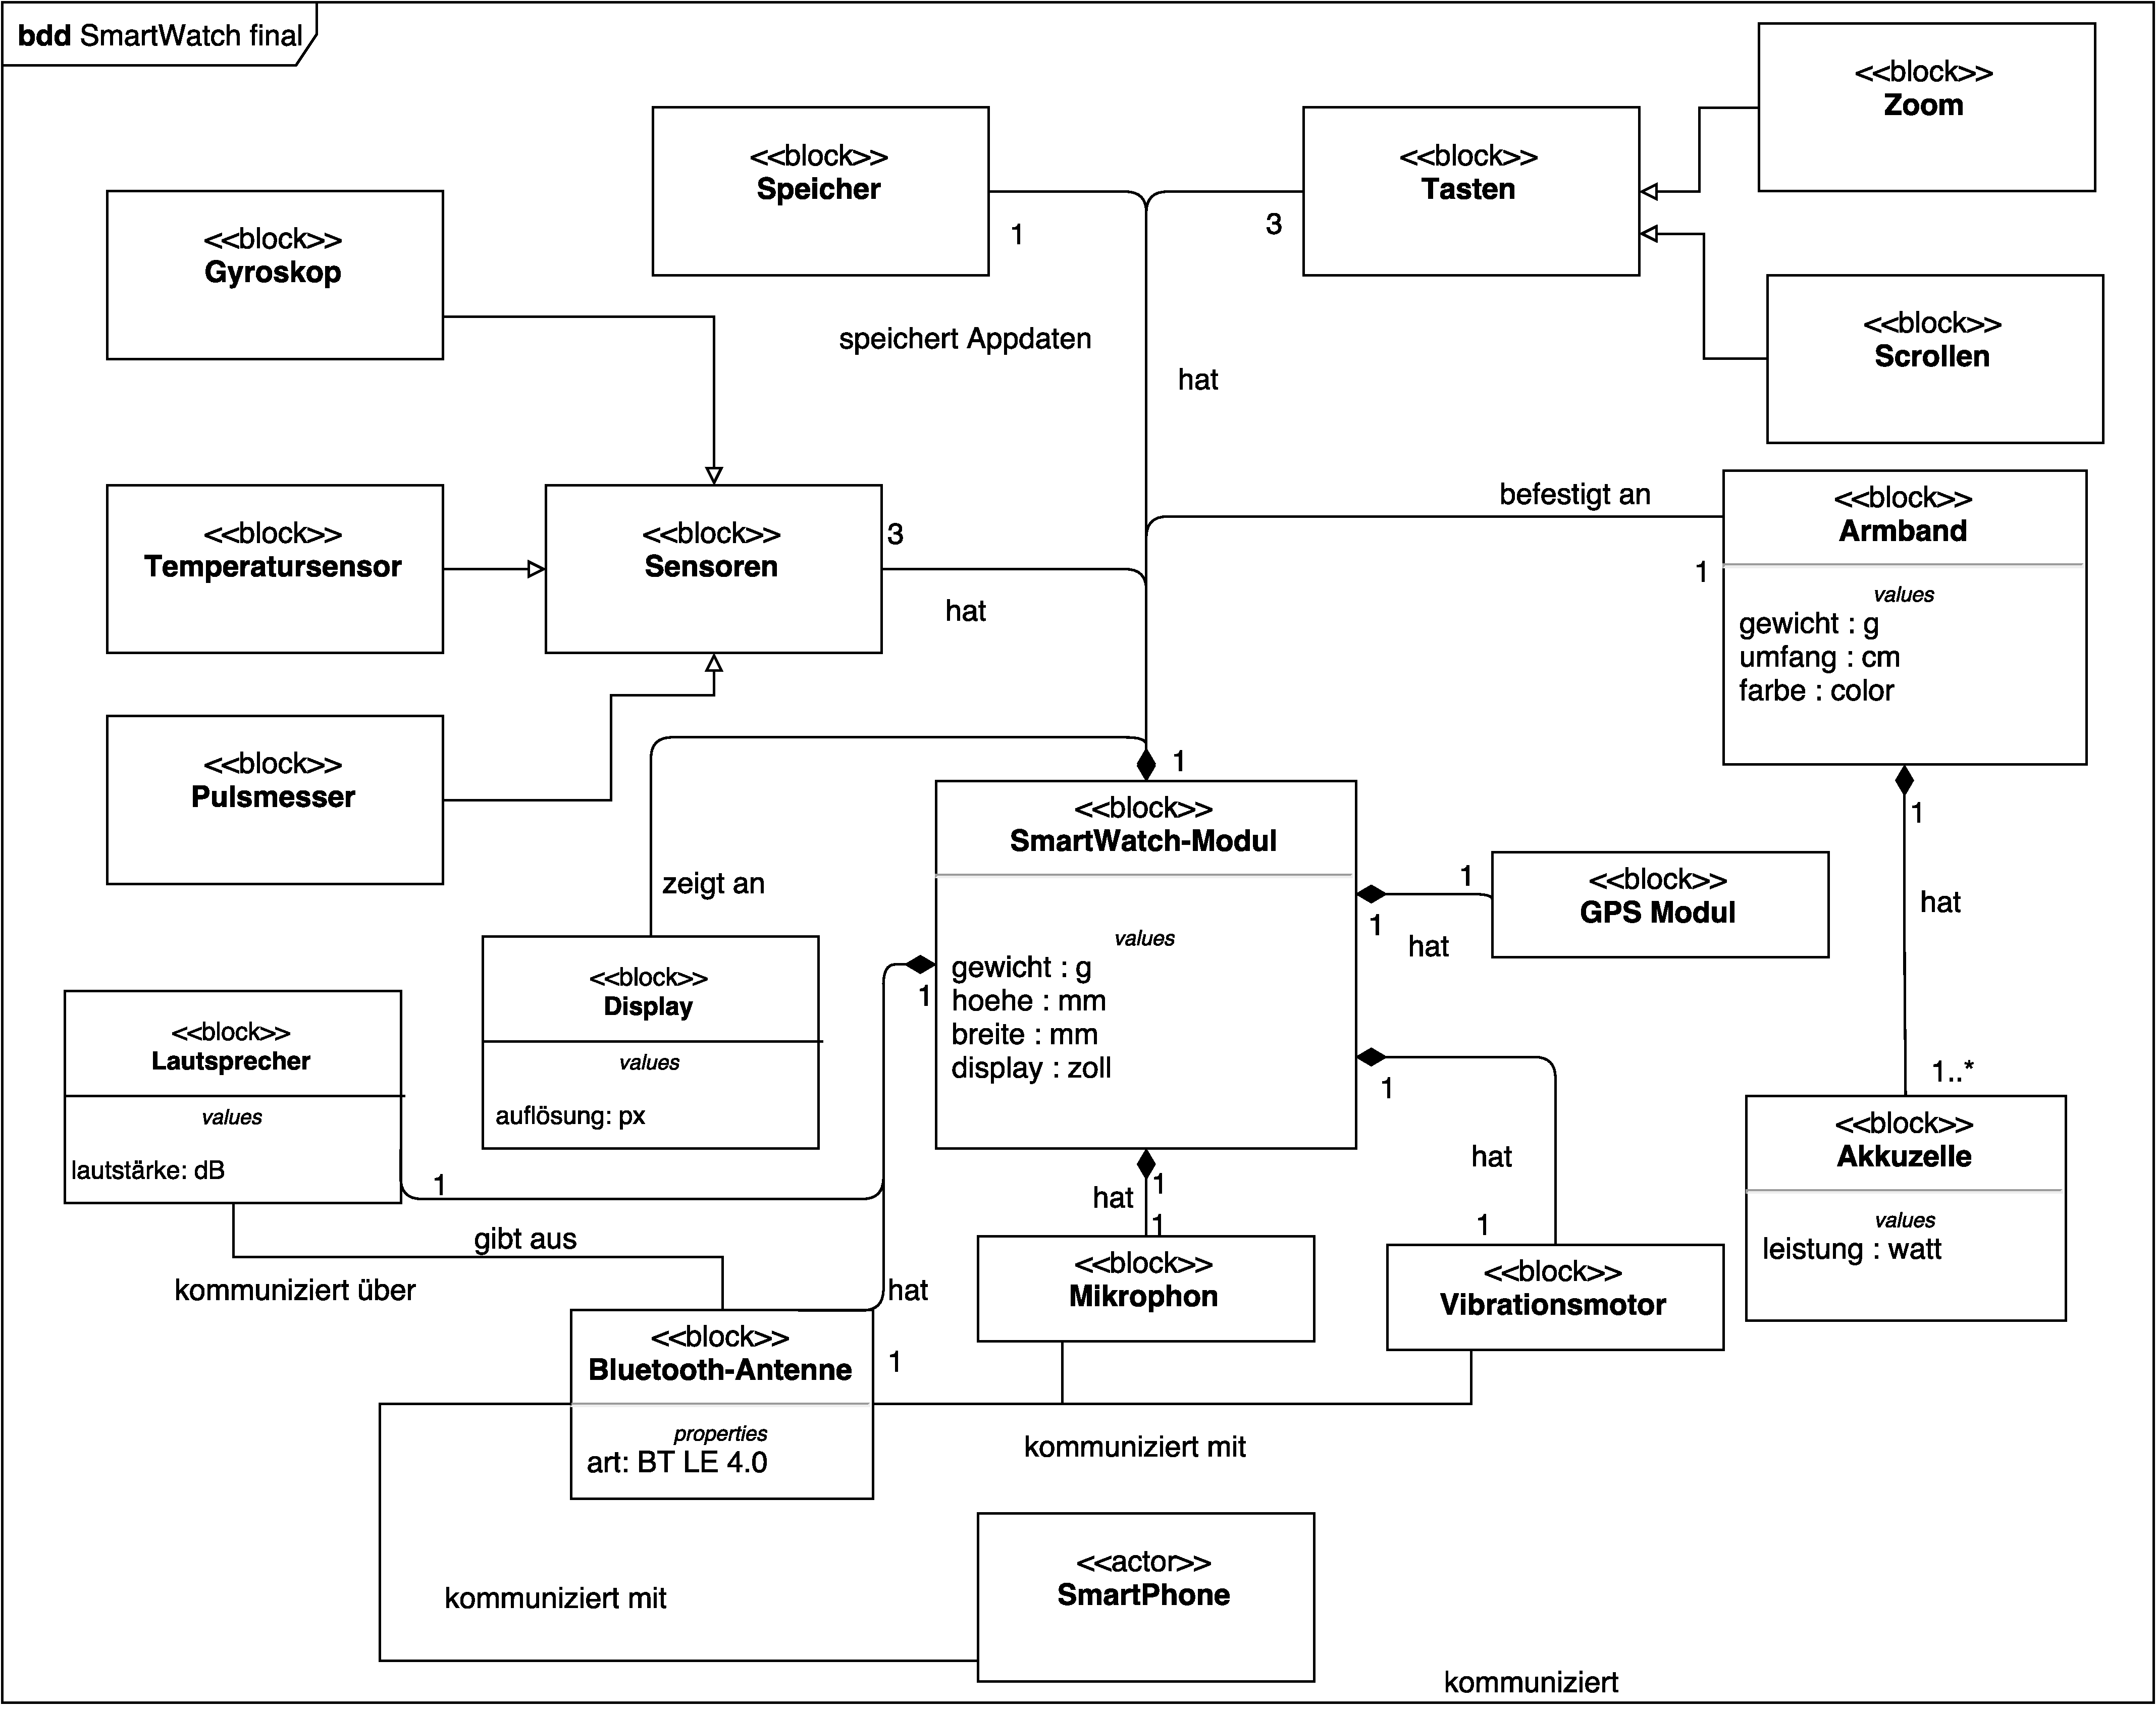
\includegraphics[width=\textwidth]{img/block2}
\caption{Endgültiger physikalischer Aufbau der SmartWatch in Phase 3 anhand eines Block Definition Diagram.}\label{fig:block2}
\end{figure}